\documentclass[a4paper,10pt]{article}
\usepackage[T1]{fontenc}
\usepackage[utf8]{inputenc}
\usepackage{lmodern}
\usepackage{url,csquotes}
\usepackage{fancyhdr}
\usepackage{graphicx}
\usepackage{epstopdf}
\usepackage{lastpage}
\usepackage{listings}
\usepackage{fancyref}
%\usepackage{subfigure}
\usepackage{enumitem}
\usepackage{tabularx, booktabs ,multirow}
\usepackage{mathtools}
\usepackage{caption}
\usepackage{subcaption}
\captionsetup{justification=centering}
\usepackage{anysize} %%pour pouvoir mettre les marges qu'on veut 
\marginsize{2cm}{2cm}{2cm}{2cm} 

\usepackage{amsfonts,amssymb,amsmath,amsthm} 
\newcommand{\vect}[2]{ \begin{bmatrix} #1 \\  #2 \end{bmatrix}  }
\newcommand{\un}{ \mathbf{1}   }
\newcommand{\zero}{ \mathbf{0}   }
\newcommand{\diag}{ \textbf{diag}   }
\newcommand{\matrice}[3]{ \begin{bmatrix}  #1 &  #3 \\ #3^T  & #2 \end{bmatrix}   }

\newcommand{\norm}[1]{\left\lVert #1 \right\rVert} 
\newcommand{\norme}[1]{\left\lVert #1 \right\rVert_2} 
\newcommand{\fsurg}{\frac{f}{g}} 
\newcommand{\prodv}[2]{ #1^T #2 } 

\usepackage{enumitem} 

% Graph package
\usepackage{tikz}
\usetikzlibrary{arrows}

\begin{document}


\begin{center}
\rule{\textwidth}{3pt}
Master MVA \\
Probabilistic Graphical Models \\
HM2 - 21/11/2016 \\
\textsc{ Achari Berrada Youssef} \\
\rule{\textwidth}{.3pt}
\end{center}

\section{Entropy and Mutual Information}
\begin{enumerate}
\item $X$ a discrete variable on a finite space $\mathcal{X}$ of cardinal $k$. 
\begin{enumerate}
\item We know that the entropy is 
\[ 
H(X) = - \sum_{x \in \mathcal{X}} p(x) \log(p(x))  \geq 0
\]
Because $0 \leq p(x) \leq 1 \Rightarrow \log(p(x)) \leq 0 \Rightarrow p(x) \log(p(x)) \leq 0 $, $\forall x \in \mathcal{X} $. \\   
So the entropy is greater than or equal to zero. \\ 
If $H(X) = 0$, then $\forall x \in \mathcal{X} , \quad p(x) \log(p(x)) = 0 \Rightarrow \forall x \in \mathcal{X} ,  p(x) = 1 \, \text{or} \, p(x) = 0 $ \\
As we know that $\sum_{x \in \mathcal{X}} p(x)   = 1 $, so we conclude that $\exists \, x \in \mathcal{X} \text{ such that } \, p(x) =1$ and null elsewhere. So X is constant. 

\item Let $q$ be the uniform distribution over $\mathcal{X}$. 
We have 

\begin{align*}
D(p||q)  & = \sum_{x \in \mathcal{X} } p(x) \log\left( \frac{p(x) }{q(x)} \right)  \\
		& = - H(X) + \log(k) 
\end{align*}

\item So we deduce from a) and b) that : 
\[ D(p||q) \leq \log(k) \]
\end{enumerate}
\item 
\begin{enumerate}
\item 
\begin{align*}
I(X_1,X_2)  & = \sum_{(x_1,x_2)\in \mathcal{X}_1 \times \mathcal{X}_2} p(x_1,x_2) \log\left( \frac{p(x_1,x_2)}{p(x_1) p(x_2)}\right) \\
			& = \mathbb{E}_{x_1,x_2} \left[  - \log\left( \frac{p(x_1) p(x_2)}{p(x_1,x_2)}\right) \right]  \\
-\log \text{ is convex} 		\qquad	& \geq   - \log\left(\mathbb{E}_{x_1,x_2} \left[  \frac{p(x_1) p(x_2)}{p(x_1,x_2)} \right]  \right) = -\log (1) = 0
\end{align*}

\item 
\begin{align*}
I(X_1,X_2)  & = \sum_{(x_1,x_2)\in \mathcal{X}_1 \times \mathcal{X}_2} p(x_1,x_2) \log\left( \frac{p(x_1,x_2)}{p(x_1) p(x_2)}\right) \\
				& = \sum_{(x_1,x_2)\in \mathcal{X}_1 \times \mathcal{X}_2} p(x_1,x_2) \log\left( p(x_1,x_2) \right) - \sum_{(x_1,x_2)\in \mathcal{X}_1 \times \mathcal{X}_2} p(x_1,x_2) \log\left( p(x_1)  \right)  \\
				& \qquad  - \sum_{(x_1,x_2)\in \mathcal{X}_1 \times \mathcal{X}_2} p(x_1,x_2) \log\left( p(x_2)  \right)   \\
				& = \sum_{(x_1,x_2)\in \mathcal{X}_1 \times \mathcal{X}_2} p(x_1,x_2) \log\left( p(x_1,x_2) \right) - \sum_{x_1\in \mathcal{X}_1 } p(x_1) \log\left( p(x_1)  \right) \\ 
				& \qquad - \sum_{x_2 \in \mathcal{X}_2} p(x_2) \log\left( p(x_2)  \right)   \\
	I(X_1,X_2)			& = H(X_1) + H(X_2) - H(X_1,X_2)
\end{align*}
\item Given $X_1,X_2$, we have that 
\[ 
H(X_1,X_2) \leq H(X_1) + H(X_2) 
\] 
With equality when $p_1$ and $p_2$ are independent random variables. \\
So the joint distribution of the maximal entropy is $p_{1,2} = p_1 p_2 $. 
\end{enumerate}
\end{enumerate}

\section{ Conditional independence and factorizations }

\begin{enumerate}
\item The direct implication is straight forward from the conditional independence axiom : \\

If $X \amalg Y | Z$, then $p(x |y,z) = p(x|z)$ for all pairs $(y,z)$ such that $p(y,z) >0 $. \\

For the converse, and consider a pair $(y,z)$ such that $p(y,z) >0$ and assume $p(x|y,z) = p(x|z)$, we have : 
\begin{align*}
p(x,y|z) & = p(x|y,z) p(y|z)   = p(x|z) p(y|z) 
\end{align*}
And this implies that $X \amalg Y | Z$.
\item Let's $p \in \mathcal{L}(G)$, we have : 
\[ 
p(x,y,z,t) = p(x) p(y) p(z|x,y) p(t|z)
\] 

It is not true that $X \amalg Y | T$. Following a Bayes Ball algorithm, when we shade the node T, a ball can pass from X to through Z then bounce back at Z and finally pass through Y.

\item Statement "$ X \amalg Y $ and $ X \amalg Y | Z$ then $ ( X \amalg Z$ or $Y\amalg Z)$"
\begin{enumerate}

\item $Z$ is a binary variable. Let's note $p(x|z=0) = p_0(x) $ , $p(x|z=1) = p_1(x) $ , $p(z=1) = q$ and $p(z=0) = 1-q$ with $ q \in [0,1]$.
We have : 
\begin{align}
p(x,y) & = \sum_{z}  p(x,y,z) = \sum_z p(x,y|z) p(z)  = \sum_z p(x|z) p(y|z) p(z) 
\end{align}

On the other side, 
\begin{align}
p(x,y) &= p(x)p(y) = \sum_{z} p(x|z)p(z) \sum_{z'} p(y|z') p(z') 
\end{align}

By equaling the equation (1) and (2), we obtain: 
\[ 
\left( (1-q) p_0(x) + q p_1(x) \right) . \left( (1-q) p_0(y) + q p_1(y) \right) =  (1-q) p_0(x) p_0(y) + q p_1(x) p_1(y)
\] 

\[ 
\Leftrightarrow  \qquad p_0(x) p_0(y)  + p_0(x) p_1(y) + p_1(x) p_0(y)  - p_1(x) p_1(y) = 0
\]

\[ 
\Leftrightarrow  \qquad  (p_0(x) - p_1(x) ) . ( p_0(y)  - p_1(y))  = 0
\]
\[ 
\Leftrightarrow  \qquad  p_0(x) =  p_1(x) \quad \text{or} \quad  p_0(y)  = p_1(y)  
\]

\[ 
\Leftrightarrow  \qquad  X \amalg Z \quad \text{or} \quad Y \amalg Z
\]
\item In general, the statement is not true.
\end{enumerate}

\end{enumerate}


\section{Distributions factorizing in a graph}
\begin{enumerate}
\item We know that in a DAG, G = (V,E) , we have that: 
\[ 
p(x) = \prod_{k \in V} p(x_k |x_{\pi_k})
\]

We know that $\pi_j = \pi_i \cup \{ j\}$, then we compute: 
\begin{align*}
p(x)  & = p(x_i|x_{\pi_i}) \quad p(x_j|x_{\pi_j})  & \prod_{k \in V \setminus \{i,j\}} p(x_k |x_{\pi_k}) \\
		& = p(x_i|x_{\pi_i}) \quad  p(x_j|x_i, x_{\pi_i}) &  \prod_{k \in V \setminus \{i,j\}} p(x_k |x_{\pi_k}) \\
		& =  p(x_j , x_i | x_{\pi_i}) &  \prod_{k \in V \setminus \{i,j\}} p(x_k |x_{\pi_k}) \\
		& =   p(x_j|x_{\pi_i}) \quad p(x_i|x_j, x_{\pi_i}) &  \prod_{k \in V \setminus \{i,j\}} p(x_k |x_{\pi_k}) \\
\end{align*}
Which prove that $\mathcal{L}(G) = \mathcal{L}(G')$.

\item G is a directed tree and does not contain any v-structure, hence \\$\exists ! y \in V, \text{s.t.} |\pi_y| = 0$ and $\forall x \in V \setminus \{ y\}, |\pi_x|  = 1$. \\$y$ is the root of the directed tree.\\
G' is an undirected tree hence it has only cliques of size 2, because the chromatic number of an undirected tree is 2. 

We know that 
\[ 
p(x_V) = p(y) \prod_{x \in v_y} p(x|y)  \prod_{(x_1,x_2) \in E , \neq y } p(x_2|x_1)  
\] 

So for all cliques, we define the potential funtion: 
\begin{itemize}
\item If $C = \{y,x\} $ then $\psi_C(x_C) = p(y) p(x|y)$ 
\item if $C = \{x_1,x_2\}$ such that $x_1 \neq y$ and $x_2 \neq y$ and $(x_1,x_2) \in E $, we define $\psi_C(x_C) =p(x_2 | x_1) $.  
\end{itemize}
Then we have proven that $\mathcal{L}(G) = \mathcal{L}(G')$.

\end{enumerate}

\newpage
\section{Implementation - Gaussian mixtures}

\begin{enumerate}[label=(\alph*)]
\item kMeans is sensible to the randomized centroids initialization, see figure\ref{Fig=kMeans}. 

\begin{figure*}[h!]
    \centering
    \begin{subfigure}[t]{0.5\textwidth}
        \centering
       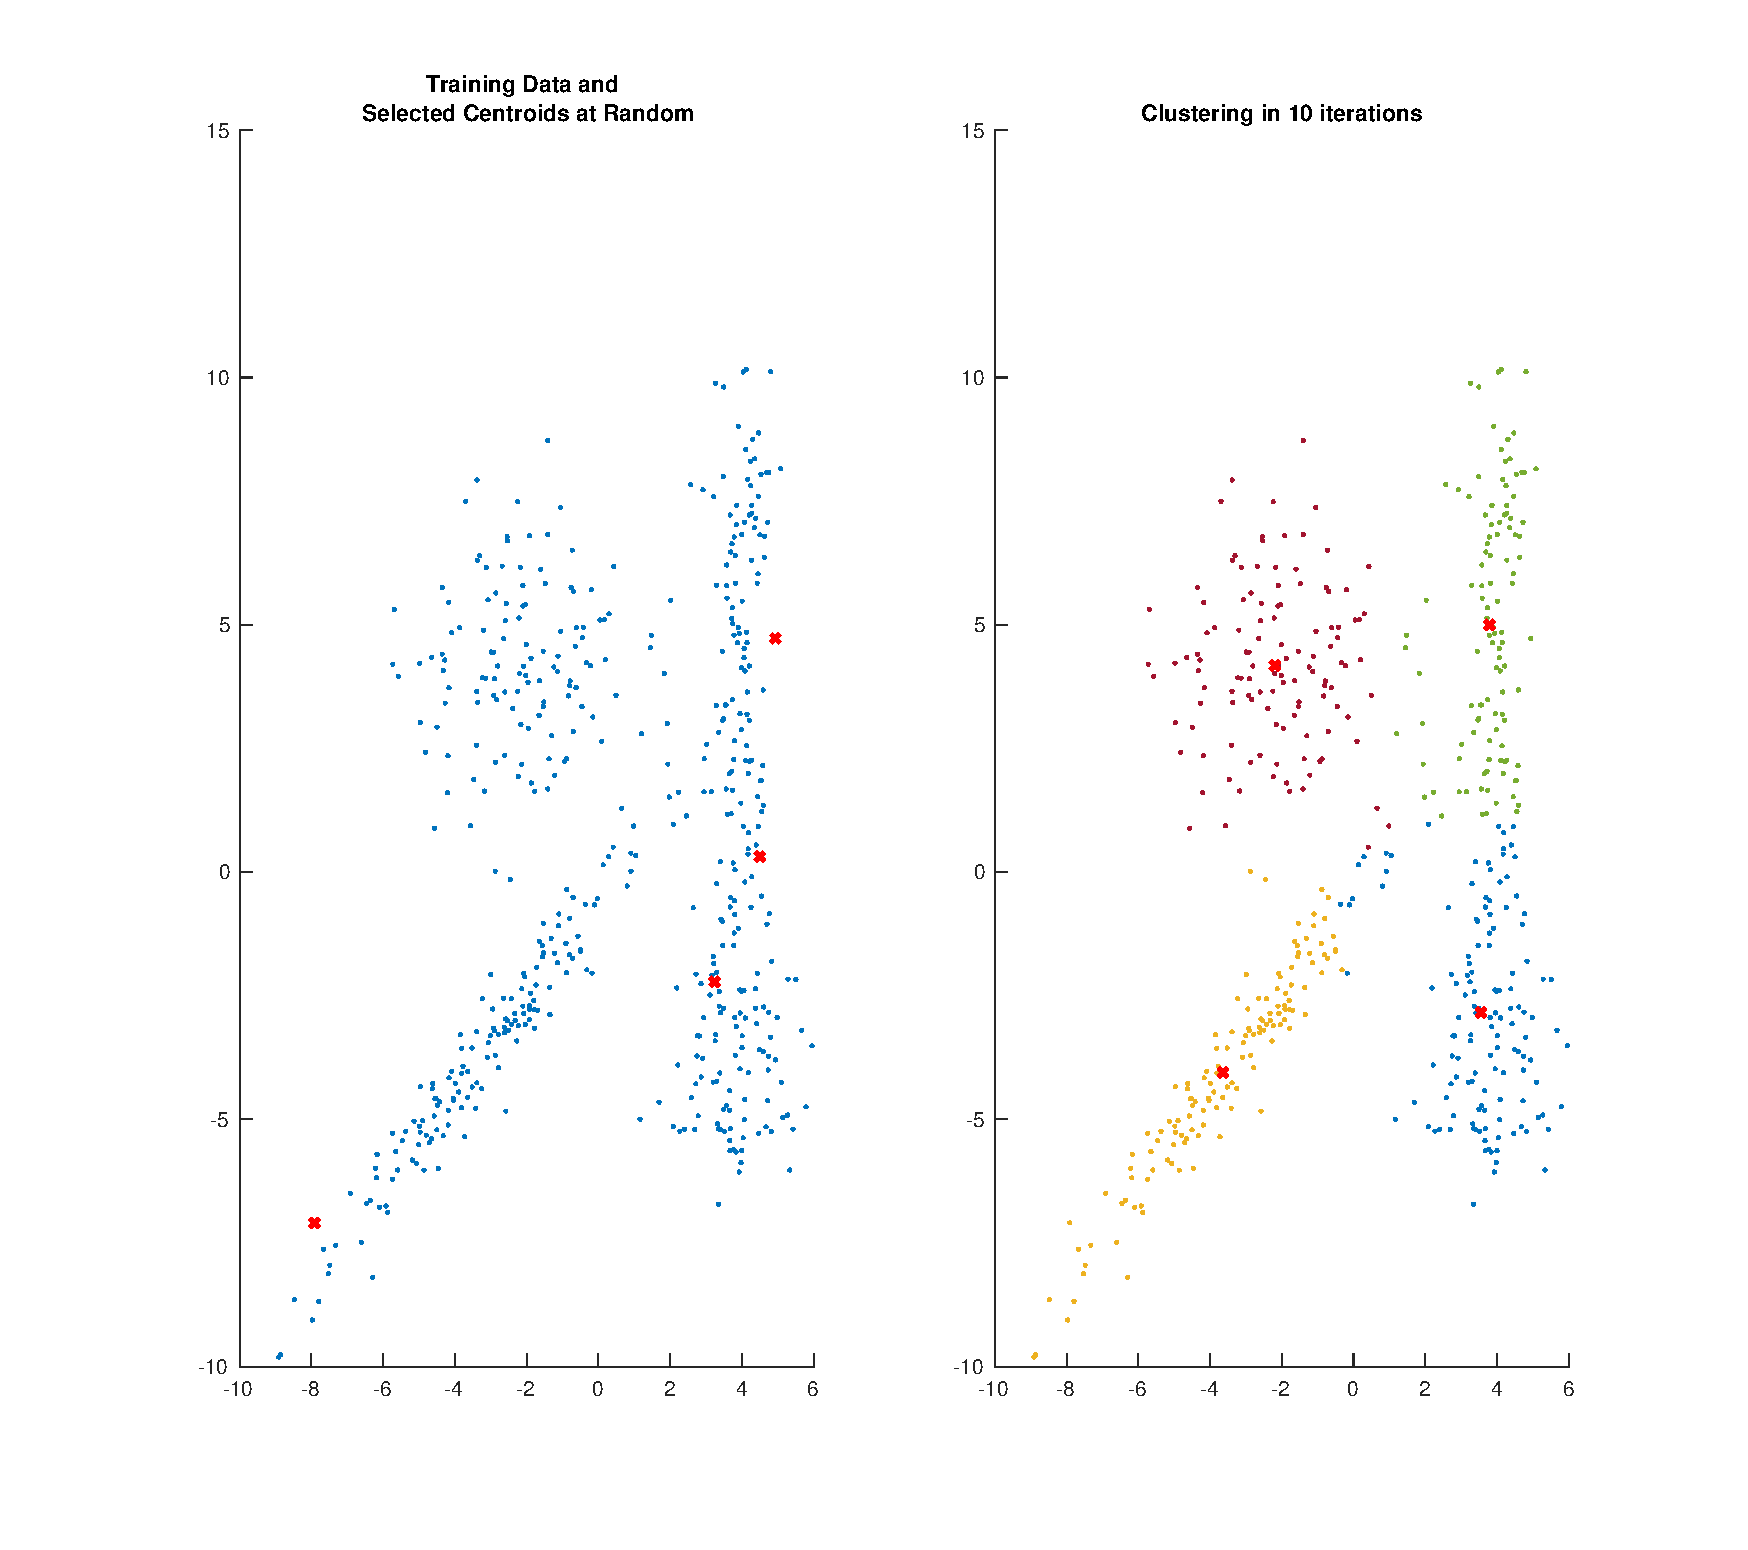
\includegraphics[width=\linewidth]{classification_data_HWK2/goodKMeans.eps} 
        \caption{Good kMeans}
    \end{subfigure}%
    ~ 
    \begin{subfigure}[t]{0.5\textwidth}
        \centering
        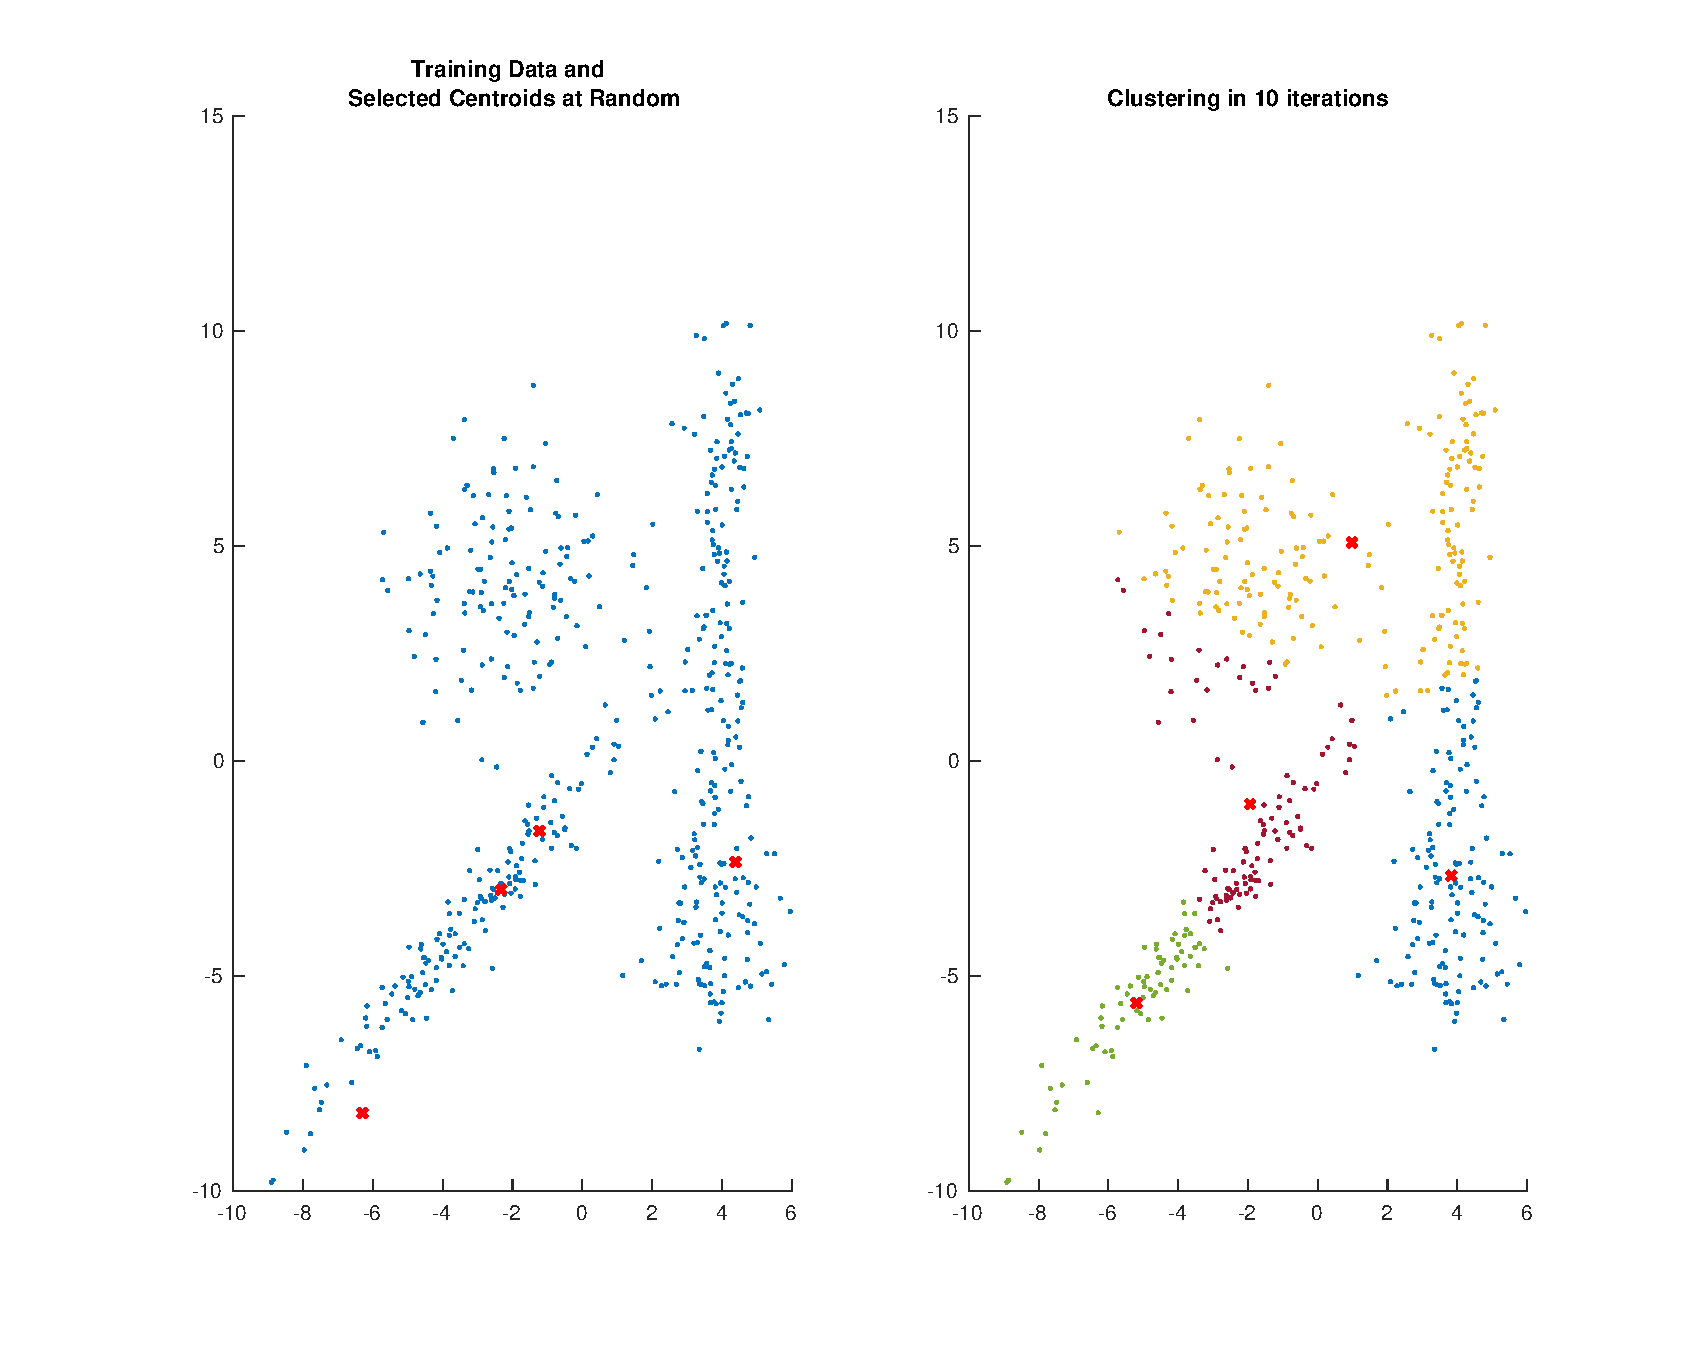
\includegraphics[width=\linewidth]{classification_data_HWK2/badKMeans.eps} 
        \caption{Bad kMeans}
    \end{subfigure}
    \caption{kMeans' sensibility on the centroids initialization} 
    \label{Fig=kMeans}
\end{figure*}

\item The parameters of the EM algorithm are: 
\[ 
 \theta   = ( \pi_k , ( \mu_k , \Sigma_k ) )_{k=1,..,K}
\]
With $ p (z) = \prod_{k=1}^K \pi_k^{z_k} \qquad$ and $\qquad p(x|z;( \mu_k , \Sigma_k )_k) = \sum_k \pi_k \mathcal{N}(x ;  \mu_k , \Sigma_k )  $ \\
\newline
We define 
\[ 
q(z) = p(z | x, \theta) \quad \, \quad \tilde{l}(\theta) = \mathbb{E}_q [\log p(x,z,\theta) ] 
\]
The goal is to maximize $  \mathbb{E}_q [\log p(x,z,\theta) ]  $. \\
First we initialize $ \mathbf{ \theta} = \mathbf{ \theta}_0$, and to do so, we use the k-Means result to estimate the parameters of the gaussians. 
At iteration $t$, we have : 
\[
q_{ik}^{(t)} = \mathbb{P}( z^{(i)}_k =1 ) = \mathbb{E}_{q_i^{(t)}} \left[z_k^{(i)} \right]
\]

\begin{enumerate}[label=\textbf{\arabic*-} ] 
\item \textbf{E}xpectation step : 
\[
q_{i,k}^{(t)} \leftarrow \dfrac{\pi_k^{t-1} \mathcal{N}(x^{(i)},\mu_k^{(t-1)},\Sigma_k^{(t)} )  }{ \sum_{j=1}^K \pi_j^{t-1} \mathcal{N}(x^{(i)},\mu_j^{(t-1)},\Sigma_j^{(t)} ) } 
\]
\item \textbf{M}aximization step : 
\[ 
\mu_k^{(t)} = \dfrac{\sum_i x^{(i)} q_{i,k}^{(t)} }{\sum_i q_{i,k}^{(t)} } \qquad , \qquad \Sigma_k^{(t)} = \dfrac{\sum_i (x^{(i)} - \mu_k )  (x^{(i)} - \mu_k )^T q_{i,k}^{(t)}  }{\sum_i q_{i,k}^{(t)}}
\]
and
\[
\pi_k^{(t)} = \dfrac{\sum_{i} x^{(i)} q_{i,k}^{(t)}}{\sum_{i,k'}  x^{(i)} q_{i,k'}^{(t)}}
\]
\end{enumerate} 

See figure \ref{Fig:CirGM} for the implementation of this methods in a particular case\footnote{I used to plot the Gaussion contour the function PLOT\_GAUSSIAN\_ELLIPSOID given by Gautam Vallabah in MathWorks.com website. }.

\begin{figure}[!h]
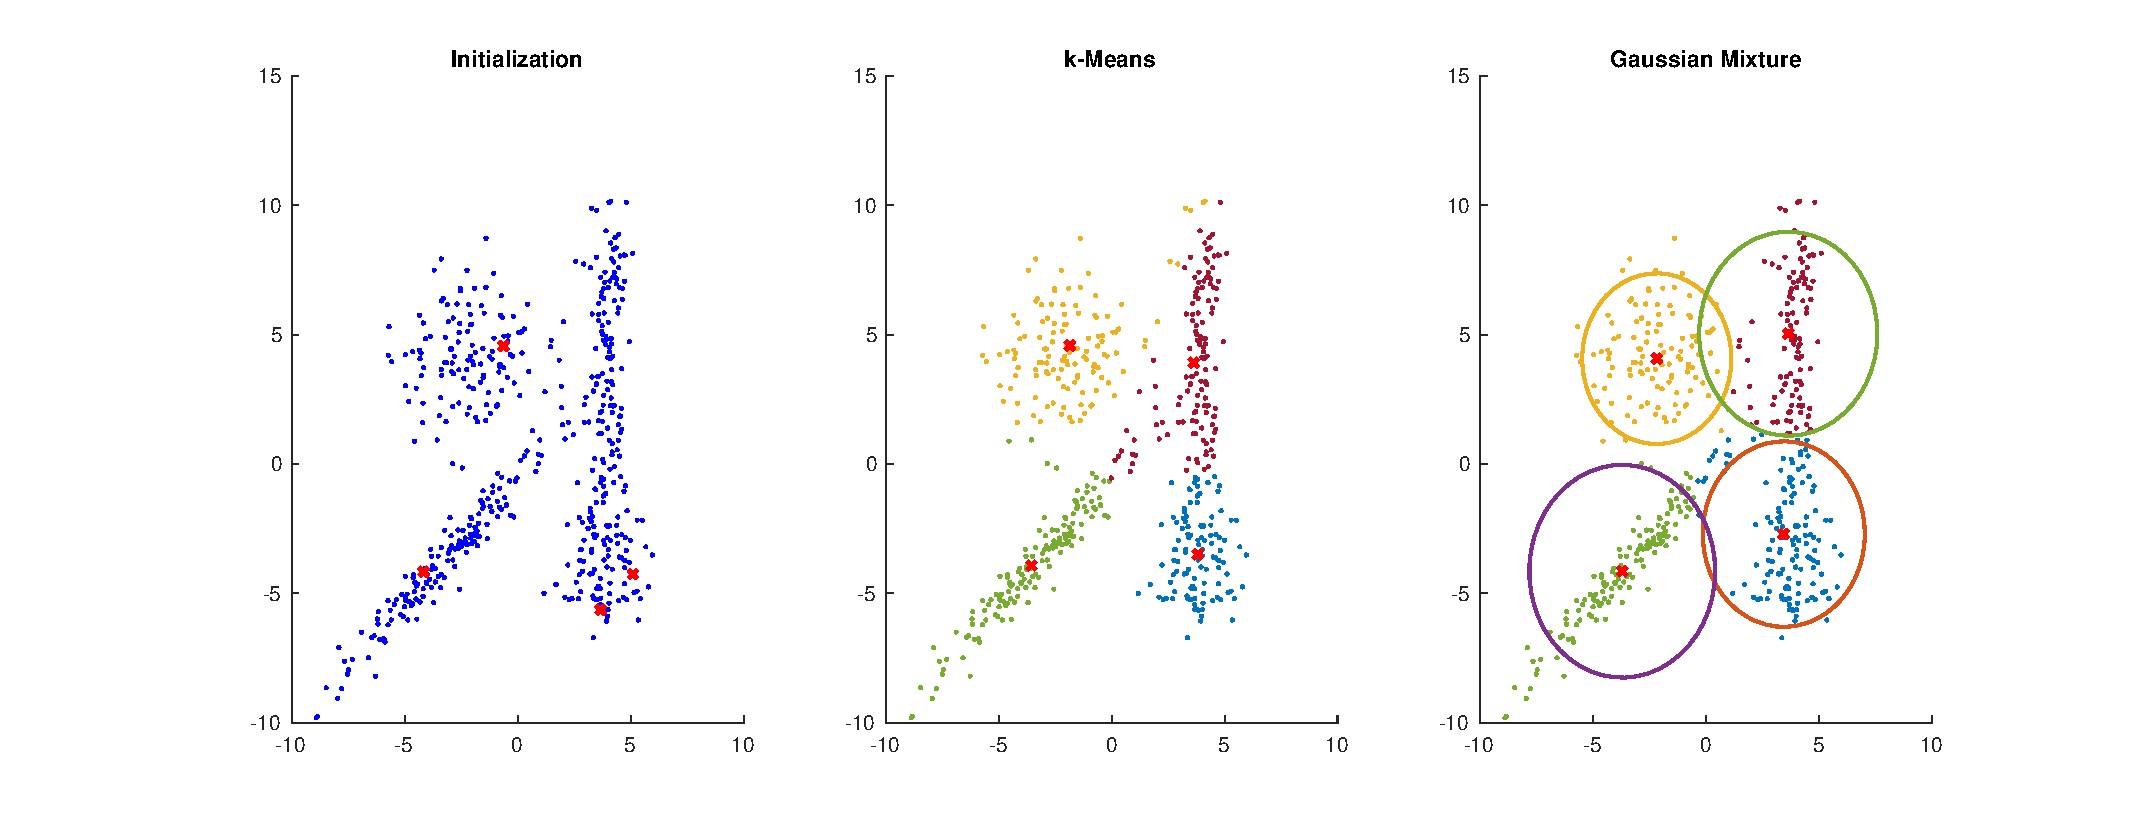
\includegraphics[width=\linewidth]{classification_data_HWK2/circleGM.eps} 
\caption{Gaussian Mixture for gaussian with covariance matrices proportional to the identity.}
\label{Fig:CirGM}
\end{figure}

\item For the general case, see figure \ref{Fig:GenGM}.

\begin{figure}[!h]
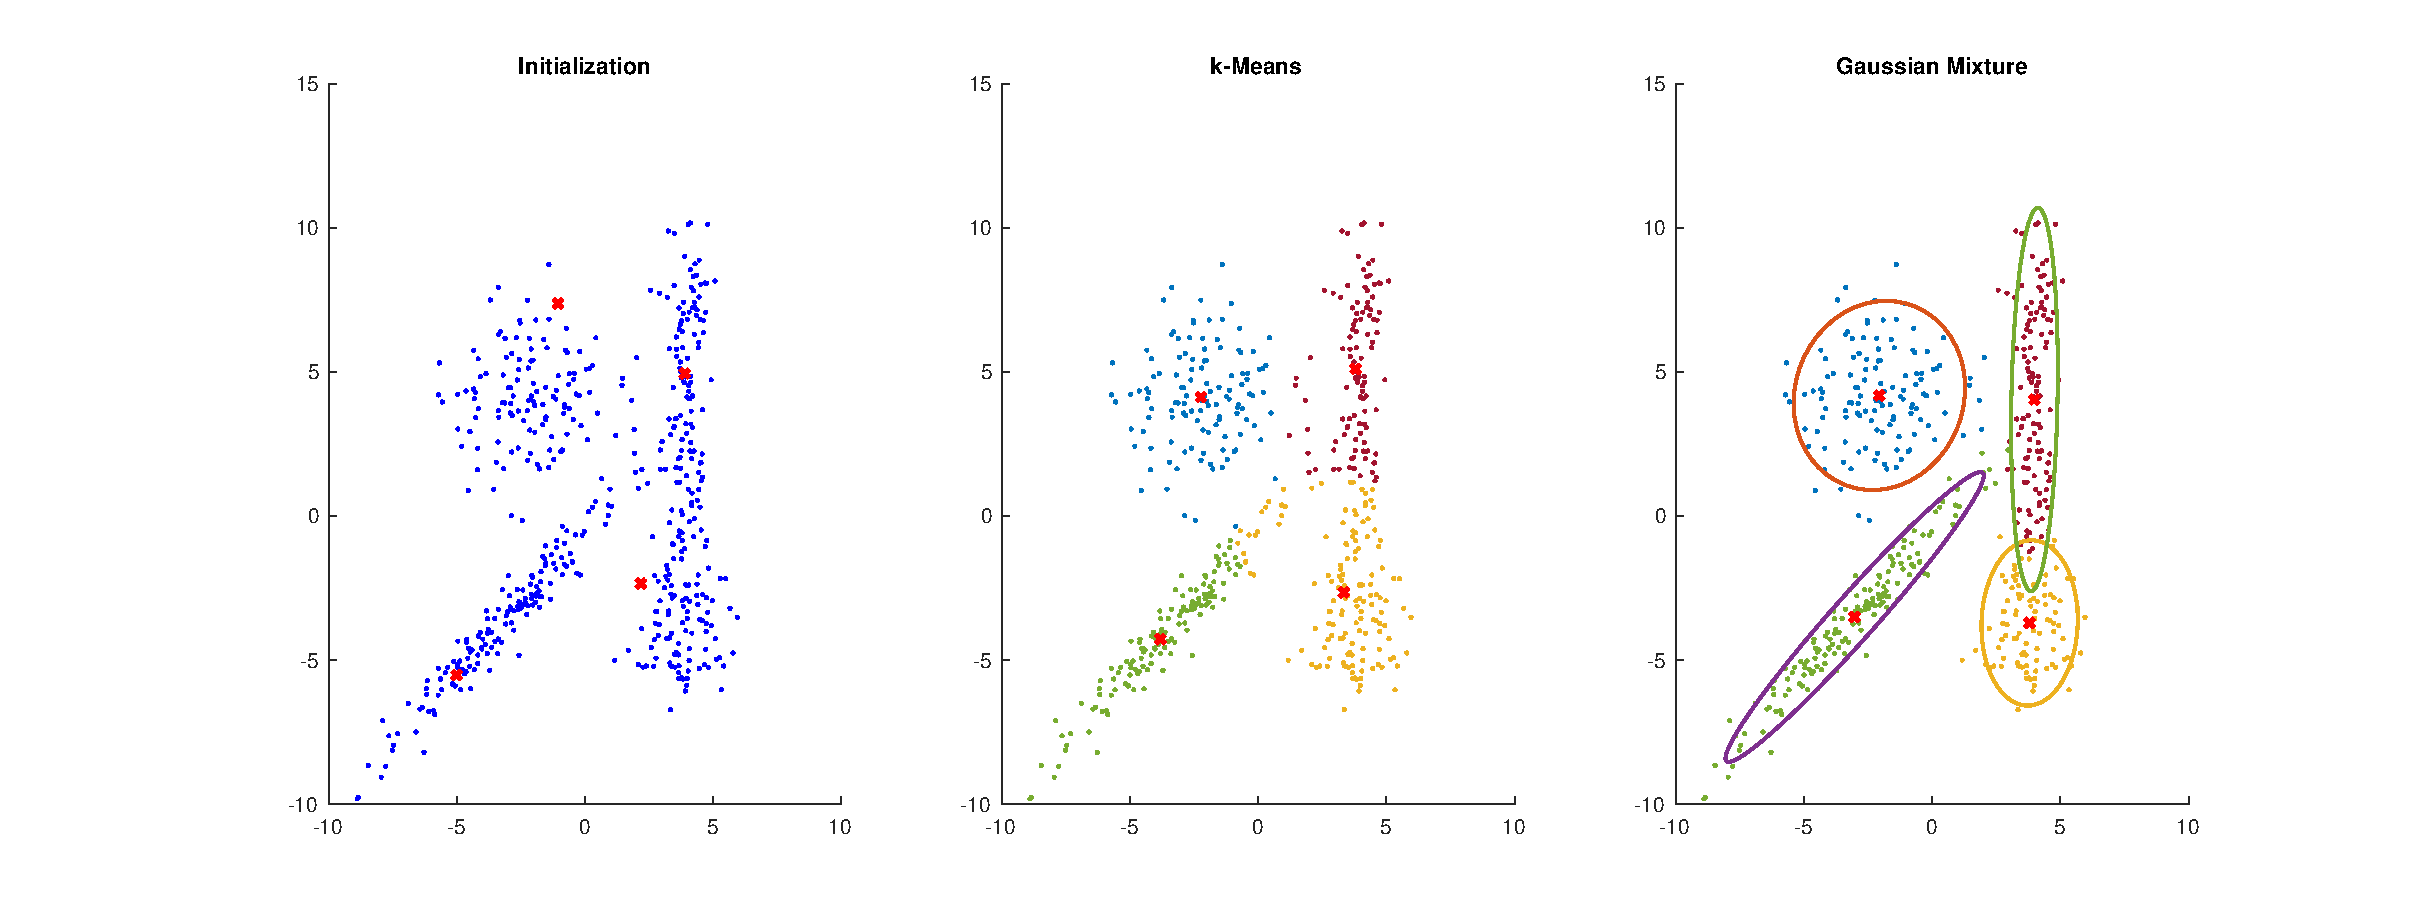
\includegraphics[width=\linewidth]{classification_data_HWK2/goodGenEM.eps} 
\caption{Gaussian Mixture for the general case.}
\label{Fig:GenGM}
\end{figure}

\item We see clearly from figures \ref{Fig:CirGM} and \ref{Fig:GenGM}, that the gaussian mixture scales better for the general case than for the limited case of identity proportional covariance matrices. This also can be seen very well in the log-likelihood estimations.

\begin{table}[!h]
\centering
\caption{Log-Likelihood Estimation.}
\label{my-label}
\begin{tabular}{lccll}
\multicolumn{1}{l|}{\begin{tabular}[c]{@{}l@{}} \end{tabular} } & \multicolumn{1}{c|}{Particular Case} & General Case         &  &  \\ \cline{1-3}
\multicolumn{1}{l|}{Training Data}                                                        & \multicolumn{1}{c|}{$3.7190$}                &           $15.6802$          &  &  \\ \cline{1-3}
\multicolumn{1}{l|}{Test Data}                                                            & \multicolumn{1}{c|}{$7.6726$}                &           $16.3715$           &  &  \\
                                                                                          & \multicolumn{1}{l}{}                 & \multicolumn{1}{l}{} &  & 
\end{tabular}
\end{table}


\end{enumerate}

\end{document}
